\documentclass[chi_draft]{sigchi}

% Use this section to set the ACM copyright statement (e.g. for
% preprints).  Consult the conference website for the camera-ready
% copyright statement.

% Copyright
\CopyrightYear{2018}
%\setcopyright{acmcopyright}
\setcopyright{acmlicensed}
%\setcopyright{rightsretained}
%\setcopyright{usgov}
%\setcopyright{usgovmixed}
%\setcopyright{cagov}
%\setcopyright{cagovmixed}
% DOI
\doi{http://dx.doi.org/10.475/123_4}
% ISBN
\isbn{123-4567-24-567/08/06}
%Conference
\conferenceinfo{ASSETS'18,}{October 22--24, 2018, Galway, Ireland}
%Price
\acmPrice{\$15.00}

% Use this command to override the default ACM copyright statement
% (e.g. for preprints).  Consult the conference website for the
% camera-ready copyright statement.

%% HOW TO OVERRIDE THE DEFAULT COPYRIGHT STRIP --
%% Please note you need to make sure the copy for your specific
%% license is used here!
% \toappear{
% Permission to make digital or hard copies of all or part of this work
% for personal or classroom use is granted without fee provided that
% copies are not made or distributed for profit or commercial advantage
% and that copies bear this notice and the full citation on the first
% page. Copyrights for components of this work owned by others than ACM
% must be honored. Abstracting with credit is permitted. To copy
% otherwise, or republish, to post on servers or to redistribute to
% lists, requires prior specific permission and/or a fee. Request
% permissions from \href{mailto:Permissions@acm.org}{Permissions@acm.org}. \\
% \emph{CHI '16},  May 07--12, 2016, San Jose, CA, USA \\
% ACM xxx-x-xxxx-xxxx-x/xx/xx\ldots \$15.00 \\
% DOI: \url{http://dx.doi.org/xx.xxxx/xxxxxxx.xxxxxxx}
% }

% Arabic page numbers for submission.  Remove this line to eliminate
% page numbers for the camera ready copy
% \pagenumbering{arabic}

% Load basic packages
\usepackage{balance}       % to better equalize the last page
\usepackage{graphics}      % for EPS, load graphicx instead 
\usepackage[T1]{fontenc}   % for umlauts and other diaeresis
\usepackage{txfonts}
\usepackage{mathptmx}
\usepackage[pdflang={en-US},pdftex]{hyperref}
\usepackage{color}
\usepackage{xspace}
\usepackage{booktabs}
\usepackage{textcomp}

% Some optional stuff you might like/need.
\usepackage{microtype}        % Improved Tracking and Kerning
% \usepackage[all]{hypcap}    % Fixes bug in hyperref caption linking
\usepackage{ccicons}          % Cite your images correctly!
% \usepackage[utf8]{inputenc} % for a UTF8 editor only

% If you want to use todo notes, marginpars etc. during creation of
% your draft document, you have to enable the "chi_draft" option for
% the document class. To do this, change the very first line to:
% "\documentclass[chi_draft]{sigchi}". You can then place todo notes
% by using the "\todo{...}"  command. Make sure to disable the draft
% option again before submitting your final document.
\usepackage{todonotes}

% Paper metadata (use plain text, for PDF inclusion and later
% re-using, if desired).  Use \emtpyauthor when submitting for review
% so you remain anonymous.
\def\plaintitle{Leveraging Augmented Reality to Create Orientation and Mobility Apps for People with Visual Disabilities}
\def\plainauthor{First Author, Second Author, Third Author,
  Fourth Author, Fifth Author, Sixth Author}
\def\emptyauthor{}
\def\plainkeywords{visual disability; orientation and mobility; augmented reality; assistive technology; smartphone apps}
\def\plaingeneralterms{Documentation, Standardization}

% llt: Define a global style for URLs, rather that the default one
\makeatletter
\def\url@leostyle{%
  \@ifundefined{selectfont}{
    \def\UrlFont{\sf}
  }{
    \def\UrlFont{\small\bf\ttfamily}
  }}
\makeatother
\urlstyle{leo}

% To make various LaTeX processors do the right thing with page size.
\def\pprw{8.5in}
\def\pprh{11in}
\special{papersize=\pprw,\pprh}
\setlength{\paperwidth}{\pprw}
\setlength{\paperheight}{\pprh}
\setlength{\pdfpagewidth}{\pprw}
\setlength{\pdfpageheight}{\pprh}

% Make sure hyperref comes last of your loaded packages, to give it a
% fighting chance of not being over-written, since its job is to
% redefine many LaTeX commands.
\definecolor{linkColor}{RGB}{6,125,233}
\hypersetup{%
  pdftitle={\plaintitle},
% Use \plainauthor for final version.
%  pdfauthor={\plainauthor},
  pdfauthor={\emptyauthor},
  pdfkeywords={\plainkeywords},
  pdfdisplaydoctitle=true, % For Accessibility
  bookmarksnumbered,
  pdfstartview={FitH},
  colorlinks,
  citecolor=black,
  filecolor=black,
  linkcolor=black,
  urlcolor=linkColor,
  breaklinks=true,
  hypertexnames=false
}


\newcommand{\BVI}{B/VI\xspace}
\newcommand{\OM}{O\&M\xspace}

% create a shortcut to typeset table headings
% \newcommand\tabhead[1]{\small\textbf{#1}}

% End of preamble. Here it comes the document.
\begin{document}

\title{\plaintitle}

\numberofauthors{3}
\author{%
  \alignauthor{Leave Authors Anonymous\\
    \affaddr{for Submission}\\
    \affaddr{City, Country}\\
    \email{e-mail address}}\\
  \alignauthor{Leave Authors Anonymous\\
    \affaddr{for Submission}\\
    \affaddr{City, Country}\\
    \email{e-mail address}}\\
  \alignauthor{Leave Authors Anonymous\\
    \affaddr{for Submission}\\
    \affaddr{City, Country}\\
    \email{e-mail address}}\\
}

\maketitle

\begin{abstract}
With the introduction of augmented reality technology to the iOS and Android platforms, mainstream smartphones now have the ability to determine their own motion in 3D space with high accuracy.  \todo{need a connection to orientation and mobility}Here, we present our work leveraging these new capabilities to create two smartphone apps for people with visual disabilities: (1) an app that provides automatic navigation guidance when backtracking along a route and (2) an app that leverages crowdsourcing to misplaced objects.  Along with a discussion of the design of the apps themselves, we present a preliminary usability study that supports their utility.  We conclude with a discussion of the promises and limitations of augmented reality smartphone technology to create assistive apps for people with visual disabilities.
\end{abstract}

\category{K.4.2.}{Assistive technology for persons with disabilities}{Orientation and mobility tools for people who are blind or visually impaired}

\keywords{\plainkeywords}

\section{Introduction}
\todo{This paragraph feels a bit disconnected. There probably needs to be something to make it more cohesive with the rest of the paper.}
For people who are blind or visually-impaired (\BVI), improvements in orientation and mobility (\OM) have been shown to increase economic opportunity as well as psychological well-being.  While only 30\% of working-age Americans who are \BVI are employed \cite{employmentstatistics2017, kirchner1999looking} (compared with 65\% of the general population), individuals with better \OM skills have a higher likelihood of being employed \cite{crudden1998comprehensive, crudden1999barriers, leonard1999factors, o1999employment}.   Similarly, while the link between visual-impairment and depression has been well-documented \cite{rubin1994visual, rovner1996depression, hayman2007depression, heyl2001psychosocial}, several studies have suggested that it is disability rather than blindness itself that is at the root of this linkage \cite{rovner1996depression, williams1998psychosocial}.  For example, it was found that one's ability to perform daily-life tasks, such as shopping for basic necessities, was \emph{more} predictive of overall life satisfaction than was degree of vision loss \cite{williams1998psychosocial}.

Due to its high degree of importance, there is a long history of engineers creating assistive technology to empower people who are \BVI to perform \OM tasks more easily (see the \emph{Background and Related Work} section).  Here, we explore new technological developments and trends that have the potential to be utilized to create widely accessible assistive technology for \OM.  The first enabling trend is the high rate of ownership of smartphones by people who are \BVI \cite{morris2014blind}.  The availability of these devices has already had revolutionary impacts on accessibility (e.g., through GPS-based directions, OCR software).  The second driver of this trend is the introduction of high accuracy 3D-tracking capabilities into mainstream smartphones.  While the primary purpose of these modules, e.g., Apple's ARKit \cite{arkit}, Google's ARCore \cite{arcore}, is to enable augmented reality applications --- whereby virtual and real world content are mingled, e.g., by overlaying images on a smartphone video feed --- these modules can be repurposed to create very powerful assistive technology for \OM.

In this document we present our work on leveraging the augmented reality modules in modern smartphones to create assistive technologies to help users who are blind with everyday \OM tasks.  In order to design maximally impactful technologies, we employ user-centered design principles throughout the research and development lifecycle, including working longitudinally with co-designers who are \BVI.  Further, two of the study authors, who are visually impaired themselves, contributed to all aspects of the project and provided design guidance based on their personal experiences.

Our first app, \emph{Clew}, enables users to backtrack along previously traveled routes.  This app is designed to alleviate various pain points experienced by non-visual travelers (e.g., finding one's way independently after being led to a location by a sighted guide).  The second app, \emph{View Share}, utilizes crowdsourcing to enable a user to find objects and receive automated guidance to objects in cluttered environments.  In the remainder of the paper we provide some relevant background and related work on \OM assistive technology, discuss some of the algorithms that underlie the AR technology of modern smartphones, discuss our two developed apps in detail, provide preliminary usability, and finally conclude with a discussion of future challenges and promising directions of smartphone-based AR technology for people who are \BVI.   \todo{Need to sell harder in the intro once the story of the paper becomes more complete.  For example, listing out the three most important contributions of this paper.  Lay out the key differentiators with previous apps, e.g. no need to instrument the environment}

\section{Background and related work}
Engineers have long sought to use technology to improve the \OM capabilities of people who are \BVI.  Most of the early work in this area has focused on the usage of technology to help with obstacle detection and avoidance.  For example, researchers have created obstacle-detecting versions of the long cane by instrumenting it with sensors such as lasers \cite{benjamin1973new} and sonar \cite{borenstein1997guidecane}.  These sorts of devices have not achieved high adoption in the \BVI community for a number of reasons, including their cost, lack of reliability, and limited new functionality over the white cane \cite{wiener2010foundations}.

Recently, spurred, in part, by the high ownership rates of smartphones among people who are \BVI, the focus of this work has shifted from obstacle avoidance to problems such as navigation and spatial awareness.  For instance, GPS-based navigation apps, such as BlindSquare \cite{blindsquare} and Google Maps, allow users who are \BVI to navigate to destinations of interest and learn about nearby landmarks and businesses.  The combination of location awareness, as provided by GPS, along with extensive databases of businesses, streets, and points of interest have allowed these apps to provide high-quality assistance to people who are \BVI.

While incredibly useful, GPS-based apps for \OM have a number of shortcomings.  Most notably, GPSes in modern smartphones are only accurate to about $10m$ in ideal conditions (they are even worse in challenging environments such as cities) and GPS does not work in indoor environments.  To circumvent these challenges, researchers are pursuing roughly two classes of approaches.  The first is to utilize crowdsroucing, whereby people who are \BVI connect over the internet with a sighted person for on-demand assistance.  Crowdsourcing has a successful track record in the area of assistive tech for the visually impaired, including the pioneering VizWiz project \cite{bigham2010vizwiz}), the free BeMyEyes app \cite{bemyeyesaccessworld}, and the subscription-based Aira system \cite{aira} (both BeMyEyes and Aira connect a user who is \BVI with a sighted volunteer through a video chat interface).  The second class of approaches combine rudimentary (and somewhat inaccurate) motion estimation via inertial sensors (gyroscopes and accelerometers) along with special environmental infrastructure (e.g., Bluetooth-enabled location beacons or Wifi access points) that provide sporadic location cues to enable relatively accurate indoor positioning.  For instance, \cite{ganz2015percept, ganz2011percept, ganz2014percept} developed a system for navigating indoor environments using smartphone-detectable RFID tags.  Dias and her collaborators utilized WiFi fingerprinting (calibrated using a highly-precise indoor mapping robot) and dead-reckoning (using the accelerometers and gyroscopes on a standard smartphone) for indoor navigation \cite{Dias__2014_7778}.  A similar system uses low-energy Bluetooth beacons instead of WiFi access points as landmarks \cite{ishihara2017beacon, ahmetovic2016navcog, ahmetovic2017achieving}.  A third approach utilizes a calibrated database containing images at known locations, which are then matched to camera images at run time \cite{bai2014wearable}.\todo{figure out a place to integrate some of Aaron Steinfeld's work}

\section{Augmented Reality}

\begin{figure}
\begin{center}
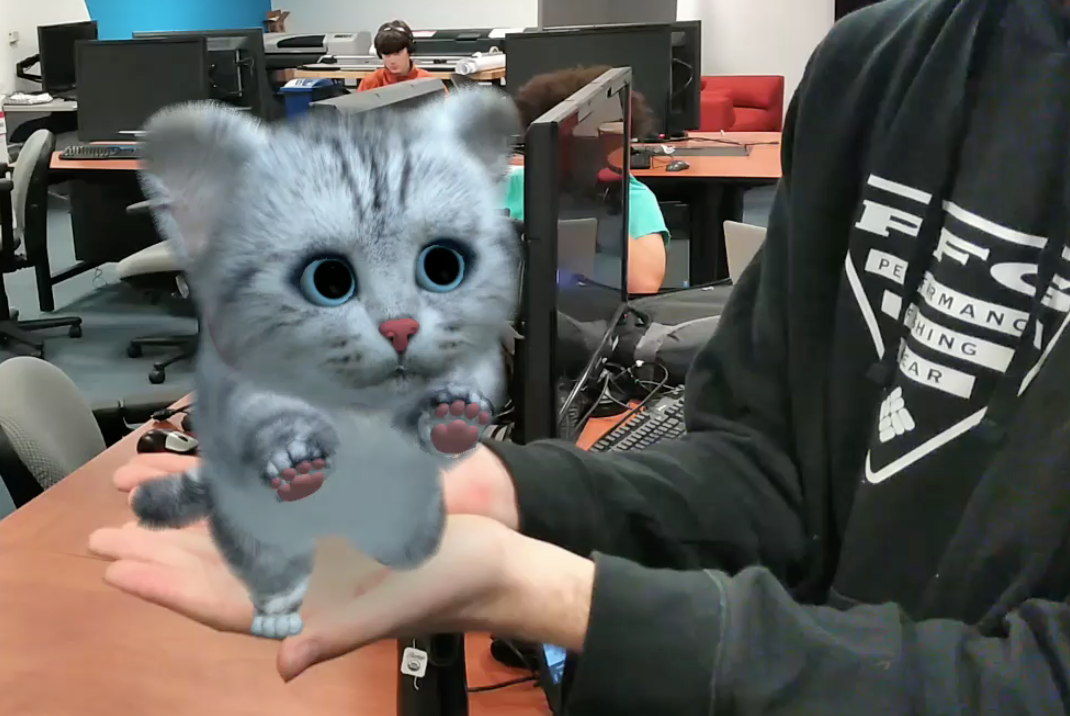
\includegraphics[width=.9\linewidth]{Figures/arexample.png}
\end{center}
\caption{A virtual cat overlaid on a smartphone camera feed.  The phone is able to accurately sense its movement in order to render the cat at the appropriate viewing angle and depth.\label{fig:arexample}}
\end{figure}

Recently, both Apple and Google have released significant new capabilities that enable users to enjoy highly sophisticated augmented reality (AR) experiences on their smartphones.  The key characteristic of AR-enabled apps is that virtual and real world content are seamlessly combined.  The most common instantiation of this idea is to overlay virtual objects or characters on a smartphone's video feed.  For instance, Figure~\ref{fig:arexample} shows a virtual cat projected into a real world scene.  As the user moves around in space, the phone senses the user's motion with high accuracy and will render the image of the cat at the appropriate distance and viewing angle, providing the illusion that the cat exists in the physical world.

These AR systems are made possible by spatial processing algorithms that are vastly more accurate than the simple inertial-based systems utilized in pervious assistive \OM apps.  The high accuracy of these systems has been driven by two key trends: the development of sophisticated algorithms for visual-inertial odometry (VIO) \cite{li2013high,leutenegger2015keyframe,bloesch2015robust,forster2014svo} (which combine optical tracking using a smartphone's camera with inertial sensing for motion estimation) and the development of special purpose hardware that allows these highly computationally intensive algorithms to run on a user's smartphone with minimal heat generation and power consumption.  The high-degree of motion estimation accuracy enabled by these systems, unlocks many new possible \OM apps for people who are \BVI, which we will described later.

\subsection{Algorithms for Visual Inertial Odometry}
In order to understand the potential of VIO for creating assistive \OM applications, it helps to understand a bit about how these algorithms function.  A full explanation of VIO is beyond the scope of this document.  For a more comprehensive treatment consult \cite{gui2015review}.  Approaches for VIO have been developed for both the stereo setting and the monocular (or single camera) setting.  The monocular setting is directly applicable to most modern smartphones, which either only have one rear-facing camera or have a second camera that is unsuitable for use in a stereo pair.  For the remainder of this section, we'll focus on the monocular case only.

VIO algorithms utilize sensor fusion to blend motion estimates generated by a camera and an IMU.  An estimate of the motion of a camera can be made by tracking salient visual features (for instance, corners or other highly textured portions of the image) over the course of multiple frames.  Utilizing the mathematics of perspective geometry, one can estimate the rotation and translation of the camera based on the global pattern of movement of these visual features \cite{Hartley2004}.  Of particular interest to the creation of assistive apps-based on this technology, the accuracy of these motion estimates is highly dependent on being able to track a large number of these visual features that ideally correspond to points at a range of distances from the camera and are distributed uniformly over the image.  This dependency means that VIO is susceptible to inaccurate motion tracking when few visual features are able to be tracked frame-to-frame or when the visual features that are tracked represent are impoverished (e.g., all at the same depth or in the same region of the image).  While some environments are simply more difficult for visual tracking, in some cases users may hold their phones in a suboptimal position (e.g., with the camera facing the ground).  Assuming a suitable set of visual features is tracked, the motion estimates of the translation of the camera are only determined up to an arbitrary scale factor.  This problem is known as scale indeterminacy.  This indeterminacy arises due to the fact that the depths (perpendicular distance from the image plane) of the visual features are unknown \cite{Hartley2004}.  For example, for any particular estimate of the translation of the camera, it is equally valid that the camera moved twice as far and the depths of the visual features were all twice as great.

The shortcomings of motion estimates from optical tracking, scale-indeterminacy and inaccurate performance in feature-poor environments, can be overcome (to some degree) by the fusion of inertial sensing data (gyroscopes and accelerometers).  Gyroscopes, which provide accurate estimates of angular velocity over short timescales, can be used to refine the estimate of rotation generated by visual tracking and accelerometer data can be integrated to obtain an estimate of linear velocity to overcome the scale-indeterminacy problem.  Since inertial sensors don't function optimally when subjected to extremely fast rotations or high accelerations, users need to hold their phones relatively stable to get the full benefits of VIO.

\subsection{VIO in Mass-Market Smartphones}
Both Apple and Google have released AR modules based on VIO.  Unfortunately, the precise details of the algorithms employed by each platform are not publicly available, however, there are important high-level distinctions between these frameworks for application developers to keep in mind.

\subsubsection{Google Tango}
The first devices based on the Google Tango platform were released by Google's ATAP (Advanced Technology and Projects) division in late 2014.  The Tango platform utilizes a wideangle (fisheye) camera equipped with a global shutter to enable maximally accurate visual-feature tracking.  Further, the platform includes a PrimeSense depth-sensing camera.  Two commercial products have been released based on the Google Tango platform: the Lenovo Phab2 Pro and the Asus Zenfone AR.  While the tracking capabilities of Tango devices are superior to other platforms (discussed next), the reliance of the platform on special-purpose hardware has severely limited the adoption of the technology, leading Google to suspend the project in March of 2018 \cite{tangoretired}.


\subsubsection{ARKit and ARCore}

Apple's ARKit \cite{arkit} and Google's ARCore \cite{arcore}, both released in 2017, provide AR-capabilities that do not require special purpose cameras.  Since these platforms utilize conventional cameras, the richness of visual features available for tracking is not as great as those available from the fisheye lenses of Tango-equipped smartphones.  Based on our anecdotal observation, the narrower field-of-view results in less accurate tracking performance than the Tango.  Further, since neither of these platforms have built-in depth sensing cameras, the availability of 3D information about the landmarks in the environment is limited to objects with special structure (e.g., horizontal and vertical planes).  Despite their drawbacks, importantly these frameworks are capable of running on a wider share of phones than Google Tango.  Further, given the high degree of preference for iOS devices among people who are \BVI \cite{morris2014blind}, ARKit is the primary platform of interest for researchers seeking to develop assistive apps based on smartphone AR technology.

\section{User-Centered Design Process}
\todo{might want to put this later.  The paper could run the risk of dragging at this point}
Our lab has been working to develop \OM assistive technology for the last several years.  We take a user-centered approach in which we deeply engage with people who are \BVI to understand their needs, wants, and values as well as any pain points and areas of opportunity that exist within their daily lives.  As such, we've used a mixture of quantitative and qualitative methods to arrive at problem spaces along with ideas for assistive technologies to help with \OM.

\subsection{Identified Areas of Opportunity}
Based on background research on, interviews with, and observation of individuals who are \BVI, we identified several areas of opportunity for the development of assistive apps.  The theme of high precision  indoor navigation came up repeatedly during this phase of our design process.  Further, the notion of being able to browse, e.g. in a grocery store or other public space, was often identified by our participants.  Finally, users expressed a desire to more quickly build facility in navigating, independently, through unfamiliar environments.

\subsection{Usability Factors of VIO Technology}
Based on the identified areas of opportunity, along with the availability of VIO on modern smartphones, it was natural to investigate the suitability of these approaches.  Since VIO is a sensor-fusion algorithm that relies, in part, on optical tracking, any assistive app based on VIO must requires the user leave their smartphone's camera is unoccluded.  In the designs explored in this paper, we assume that the user would hold the phone in one hand while holding their long cane in the other.  In some cases the user may require handsfree operation of their smartphone. The development of handsfree methods for utilizing VIO is an area we are actively researching.

\subsection{Participatory Design}
\todo{this is redundant with the intro... Either expand or ditch this.}
Throughout the development of the apps described in this document, we utilized a participatory approach to design.  This manifested itself in two specific ways.  First, we worked with a college student who is blind during five, three-hour co-design sessions to both develop the basic concept and test various prototypes for our \emph{Clew} app.   Second, two of the authors of this paper are themselves visually impaired.  In addition to their contributions to the design and implementation of the apps, their personal experiences helped guide the design process.

\section{Clew: automatic guidance along previously traveled routes}


\begin{figure}
\begin{center}
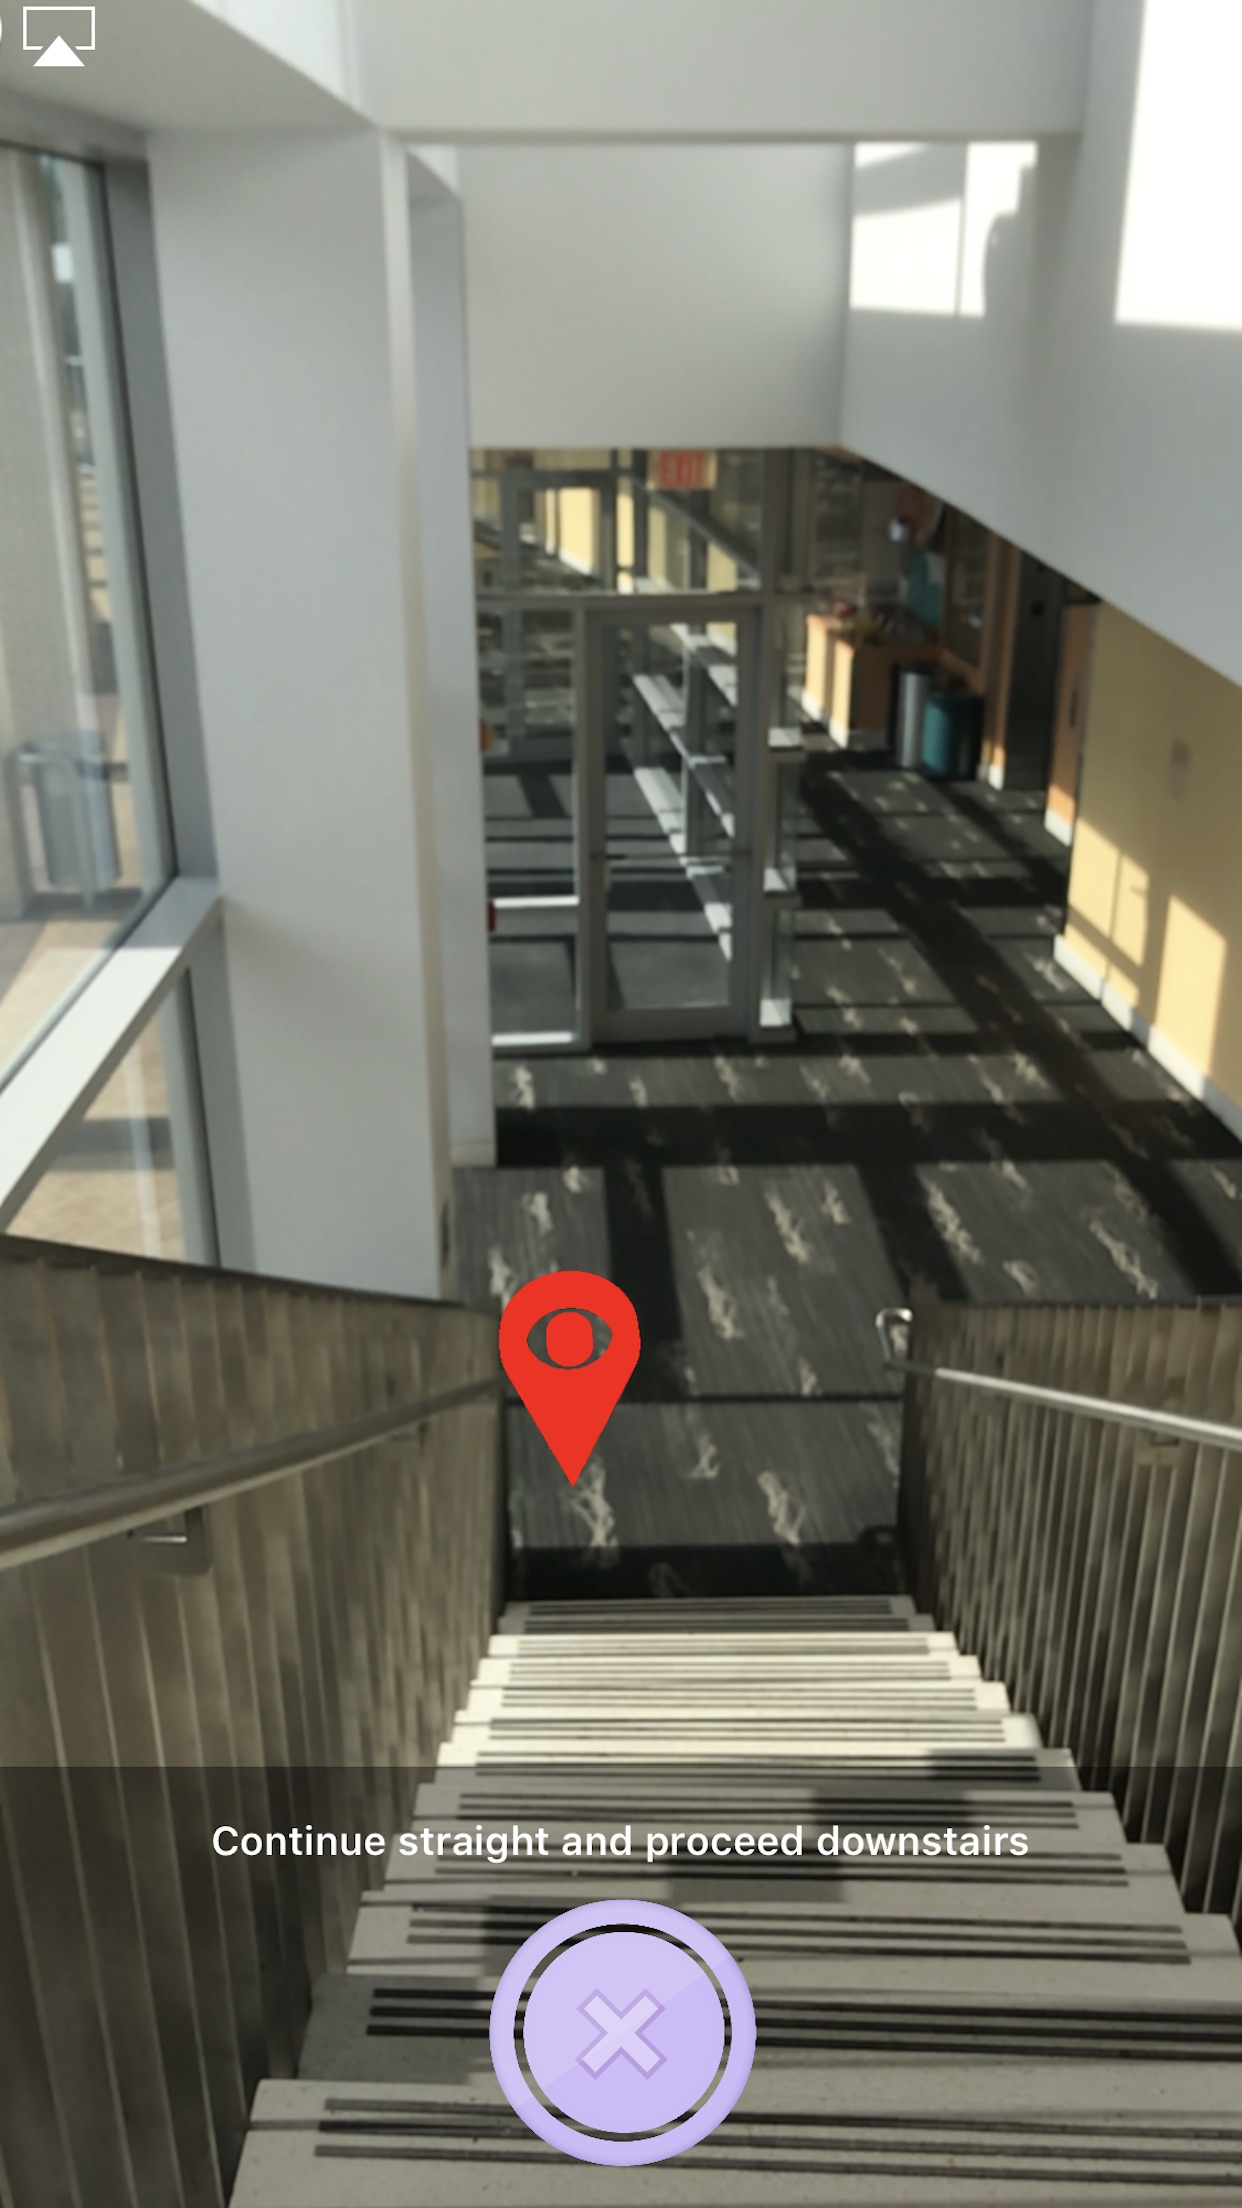
\includegraphics[width=0.48\linewidth]{Figures/clew_screenshot_1}\hspace{.03\linewidth}
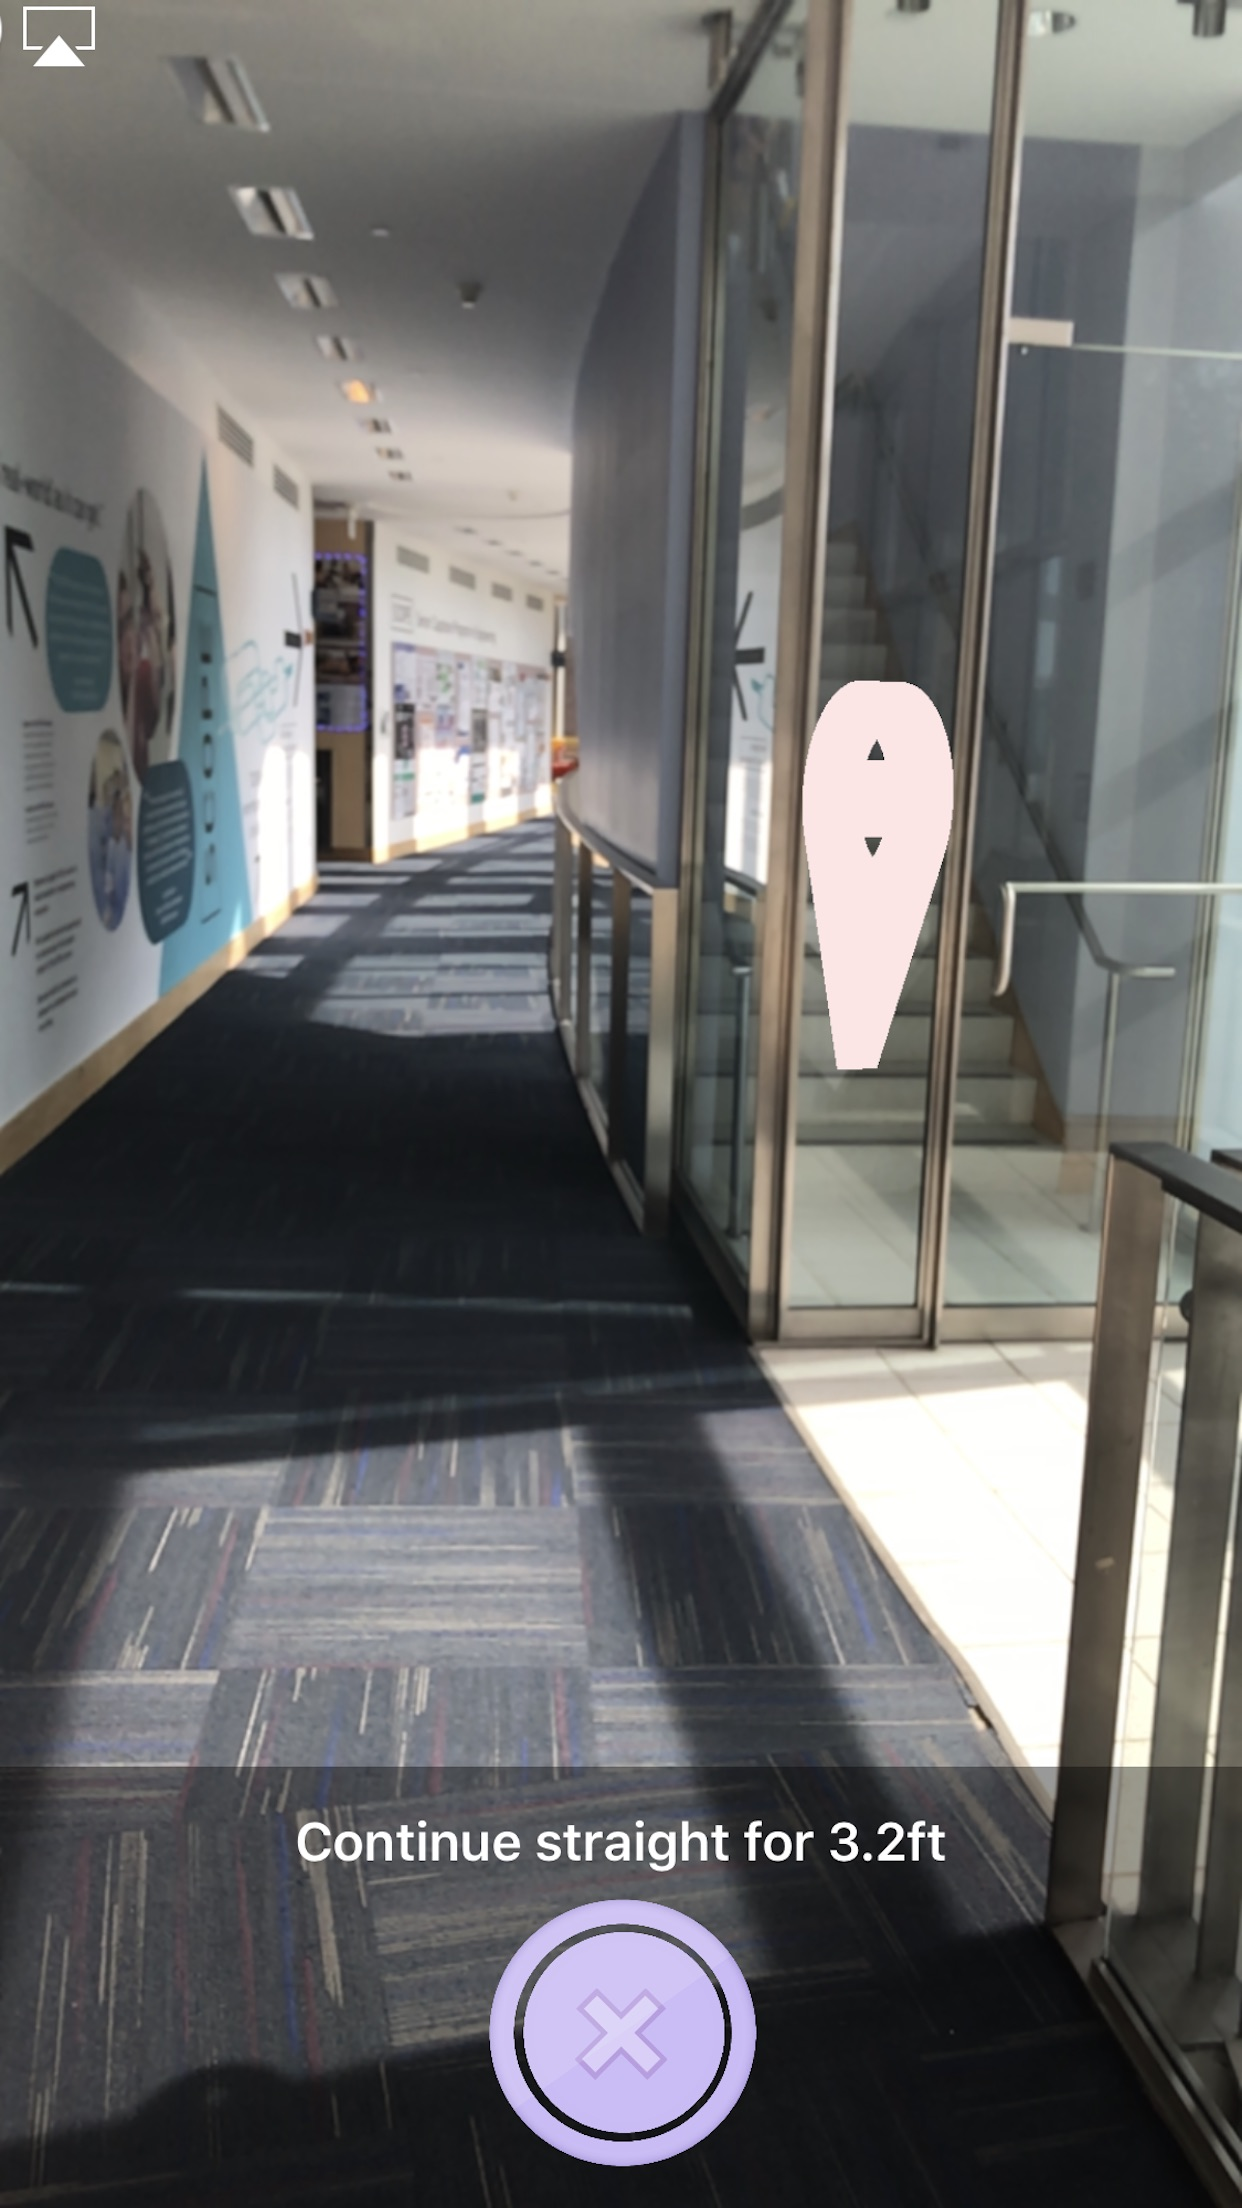
\includegraphics[width=0.48\linewidth]{Figures/clew_screenshot_2}
\end{center}
\caption{Two screenshots from our app ``Clew.'' Both images show the app in navigation mode where a user is using the app to retrace a route they have previously traveled.  The text for the left image says ``Continue straight and proceed downstairs'' and the text on the right says ``Continue straight for 3.2 feet.''\label{fig:clewshots}}
\end{figure}

\begin{figure*}
\begin{center}
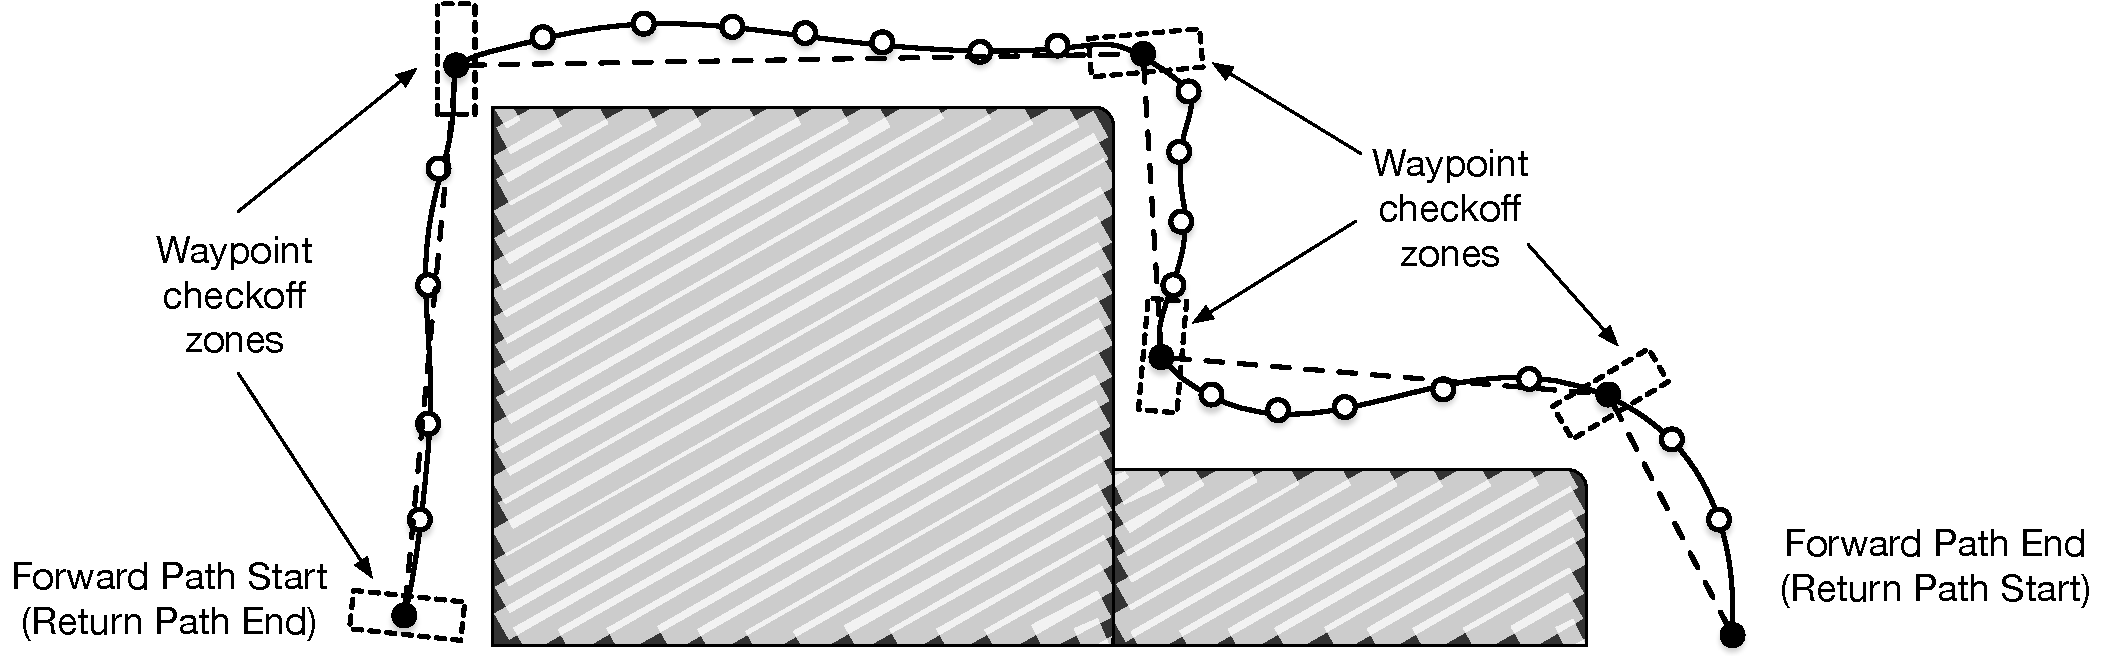
\includegraphics[width=0.9\linewidth]{Figures/samplepath}
\end{center}
\caption{A topdown view of a sample path generated by the \emph{Clew} app.  The raw path shown as a solid line is sampled, in time, as a trail of virtual breadcrumbs (white circles with black outlines).  The Ramer-Douglas-Peucker algorithm is applied to reduce the breadcrumbs to a more manageable number of waypoints (solid black circles).  The resultant path consists of straight lines connecting these waypoints in reverse time order (since the user will be navigating the path in reverse).  Waypoint checkoff zones (dashed boxes) are create to be wide in dimensions perpendicular to the direction of travel and narrow in directions parallel to the direction of travel.  The light gray area filled with diagonal lines denotes a region of the space that is impassible.\label{fig:samplepath}}
\end{figure*}

We present an iPhone app called \emph{Clew} based on the ARKit platform (Clew is available on the app store, link redacted for anonymous review).  Clew provides automatic, turn-by-turn directions to guide users who are \BVI along previously traveled routes.This use case arises, primarily, in the following two scenarios.  Firstly, when a user is led to a location in an unfamiliar environment by a sighted guide, they may desire to return to their previous location at a later time --- without the need for the sighted guide to help them.  Secondly, there are examples of places that are easier someone who is \BVI to navigate out of than to navigate back to.  For instance, it is easier to leave a conference room than it is to find your way back to the particular seat that you occupied prior to leaving.  For both of these uses cases, \emph{Clew} is able to provide high-accuracy, easy-to-follow, navigational guidance to enable people who are \BVI.  Additionally, of particular importance, this app requires no environmental modification in order to work (e.g., the introduction of beacons or special signage).  

The app works by dropping a trail of virtual breadcrumbs (which represent timestamped positions), which can be followed in reverse order at a later time.  We call the phase of laying down these virtual breadcrumbs, \emph{path recording} mode.  In \emph{path recording} mode, the user holds their smartphone with the screen facing towards them and the camera facing roughly parallel to the ground (recall that ARKit is based on VIO, which requires optical tracking to function optimally).  Once path recording mode is active, the user travels to a new location (either via their traditional \OM process or via a sighted guide).  Figure~\ref{fig:samplepath} shows a sample path taken through an environment.  A virtual breadcrumb (shown as a white circle with a black outline) is dropped at a fixed time interval.

When the user is done recording their path, they can either enter a pause mode (described later) or navigate back along their route.  When navigating along back along the route, the trail of breadcrumbs is first preprocessed by the Douglas-Ramer-Peucker algorithm \cite{douglas1973algorithms} for path simplification.  This algorithm attempts to winnow down a path, represented by a discrete number of spatial points, by removing sequences of points that can be faithfully represented by a single straight line.  In Figure~\ref{fig:samplepath}, the breadcrumbs selected for the simplified path are shown as black circles, and the resultant  straight line path is shown as a black dashed line.  The selected breadcrumbs are called \emph{waypoints}.  In \emph{navigation mode}, the app synthesizes directions to the next waypoint using one of three feedback mechanisms: (1) speech (e.g., ``continue straight for 10 feet'', (2) haptic feedback or (3) an audible beep when the phone is pointing, approximately, towards the next waypoint.  The latency of the update of the iPhone's position is so low that when using feedback mechanism (2) or (3), the user can rapidly sweep their the phone back and forth until they feel the haptic feedback or hear the auditory cue.  Even with one sweep it is possible to sense the direction to the next waypoint with high accuracy.  Screenshots of the app in navigation mode are show in Figure~\ref{fig:clewshots}.

As the user navigates, the app continuously checks to see if the user has reached the next waypoint.  We define the condition of ``reached the next waypoint'' as the user entering a \emph{waypoint checkoff zone} (labeled in Figure~\ref{fig:samplepath}).  Instead of making these checkoff zones spherical, we chose to make them rectangular prisms where the side length for the dimensions perpendicular to the direction of travel from the previous waypoint are greater than for dimensions parallel to the direction of travel.  This choice of checkoff zone shape enables the user to deviate laterally from the intended path without missing a waypoint.  The app also handles the user going up or down stairs by specially marking waypoints as belonging to a flight of stairs if the vertical angle of the segment connecting two waypoints exceeds a threshold.

\subsection{Pause feature}
In order for an ARKit tracking session to function properly, the user must not switch to a different app, lock the phone, or block the camera.  This can be a hindrance in situations where the user wants to wait a significant amount of time between traveling to a destination and navigating back, when the user would like to use some other app on their phone, or when the user needs both of their hands to perform some set of tasks before the return trip.  ARKit does support a pause feature for a tracking session, however, when the session is unpaused the phone's position, as reported by ARKit, will remain the same as when it was initially paused.  Given this limitation we designed our pause feature to prompt the user to place the phone in an position and orientation before pausing that will be easy to recreate when the user unpauses the app.  Features such as walls or doors work well for this purpose.  It is not as crucial that the user is able to exactly recreate the position and orientation at pause time.  Of all of the components of the phone's pose, the most important to recreate is the phone's yaw (see Figure~TODO).  The reason for this is that the phone's accelerometer can easily determine the other two degrees of freedom of rotation (as these are not perpendicular to gravity) and small changes deviations in the phone's position will cause a fixed amount of error, whereas an error in the phone's yaw will be magnified the farther the user travels (see Figure~TODO).

\subsection{Co-design process}
The \emph{Clew} app was developed, refined, and tested in collaboration with a college student with Retinitis Pigmentosa, a vision disorder that leads to the loss of peripheral vision to the point where someone eventually has little to no functional vision.  Weekly, over the course of five weeks, our co-design partner shaped the creation of the app and provided suggestions for improvements as well as usability enhancements.

\subsection{Usability testing}
TBD.

\section{ViewShare: Object Finding in Challenging Environments}

Object-finding in unfamiliar environments can be very challenging for people who are \BVI \todo{citation needed}.  Researchers have attempted to build systems that could enable people who are \BVI to more easily find objects whose locations are unknown (either because the location was never known to begin with or because the objects were moved by a third party).  Inspired by previous work \cite{bigham2010vizwizlocateit} that utilized a crowdsourcing model, whereby sighted online volunteers labeled an object of interest and a mobile phone automatically provided sonic cues to guide a user to the object, we developed the \emph{ViewShare} app.

The ViewShare app users the following sequence of steps to provide high precision guidance to objects of interest.  First, the user, who is \BVI, launches the ViewShare app which starts a tracking location tracking session using ARKit.  Once the user is ready to find an object, they announce it, the phone recognizes their voice command using Apple's Siri kit, and a localization job is created.  This localization job is assigned to a number of sighted volunteers who are alerted via push notification on their smartphones.  On the user's device, every two seconds an image is being captured from the users smartphone and added to the localization job.  Once the volunteer clicks on the relevant push notification they see the images collected from the user's smartphone.  If they are able to locate the object of interest, they click on its position in any one of the provided images.  The location (as a 2D pixel coordinates) is relayed back to the user's app, which then attempts to convert this 2D pixel coordinate into a 3D position using the procedures outlined in the sub section below on \emph{2D to 3D Mapping}.  If a 3D location can be determined, the user is then provided with automatic guidance to the object of interest in the form of computer-generated speech and haptic feedback.

\subsection{Object Localization Feedback}
The ViewShare app generates a haptic cue when the phone is oriented towards a located object.  As discussed earlier, the low latency of this mechanism allows the user to sweep the phone around to find objects.  Further, the app can also synthesize speech feedback to the user when their phone is facing an object.  This speech feedback includes both the name of the object along with the distance to the object.  The app can provide feedback in two different modes.  The first mode is 2D position, whereby notions of distance as well as whether or not the phone is oriented towards an object are determined by projecting the 3D positions of the phone and localized objects into the floor plane.  This mode is useful for navigating to objects that are far away (e.g., farther than 10 feet).  The second mode is 3D position, whereby notions of distance as well as whether or not the phone is oriented towards an object are determined by using the unmodified 3D positions and orientations of the phone and localized objects.  This mode is appropriate for finding objects that are close by and are relatively small in terms of their vertical extant.  For example, it might be useful to use 3D mode to find a pen, whereas finding a door would be best approached using 2D.


\begin{figure}
\begin{center}
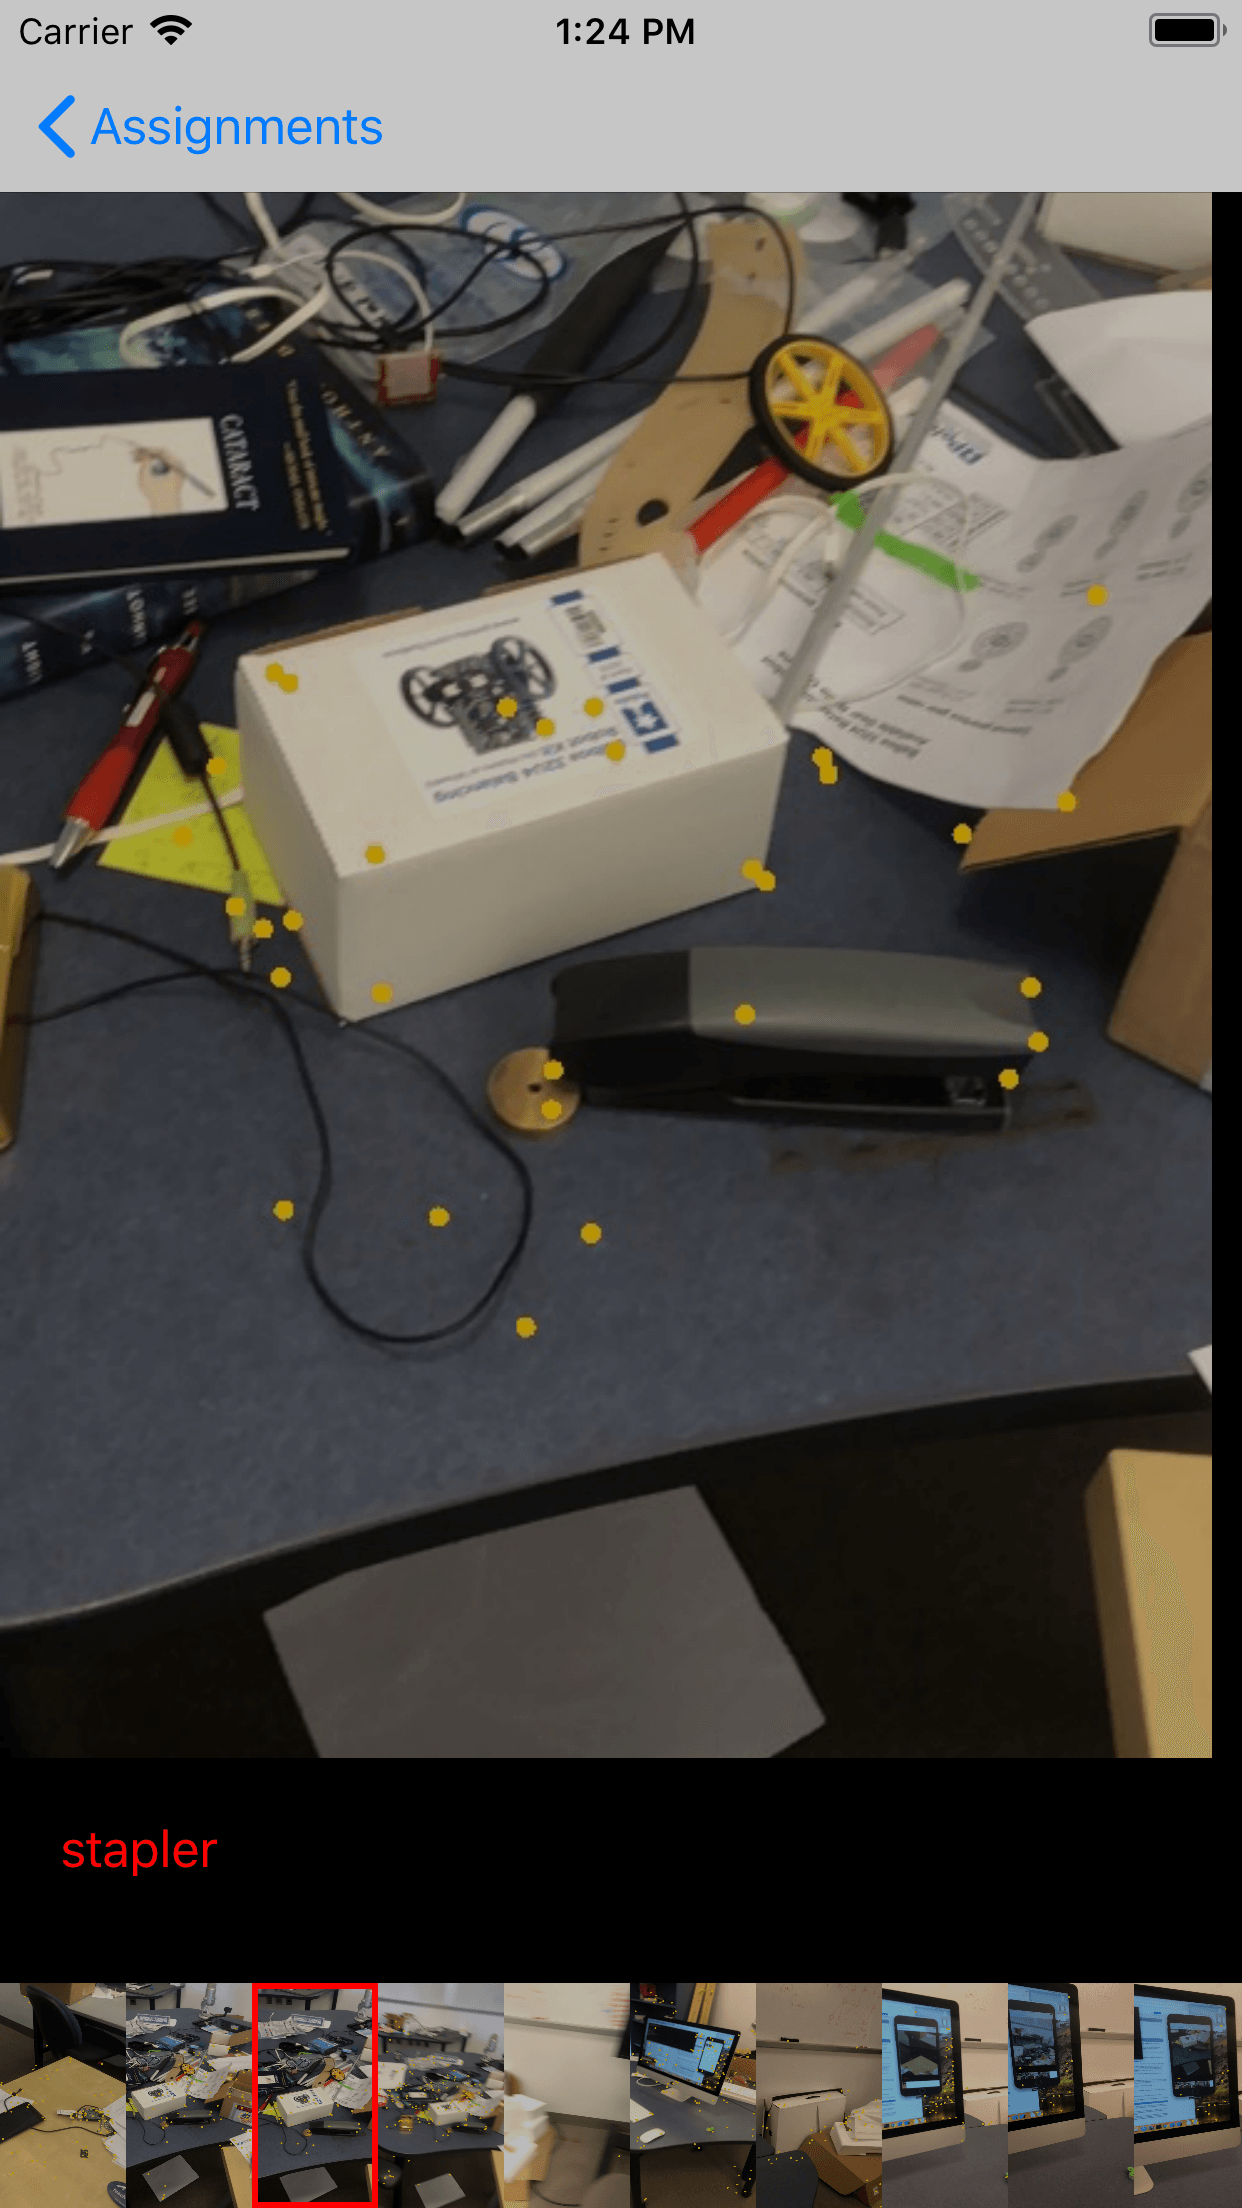
\includegraphics[height=3in]{Figures/viewshare_crowdworker}
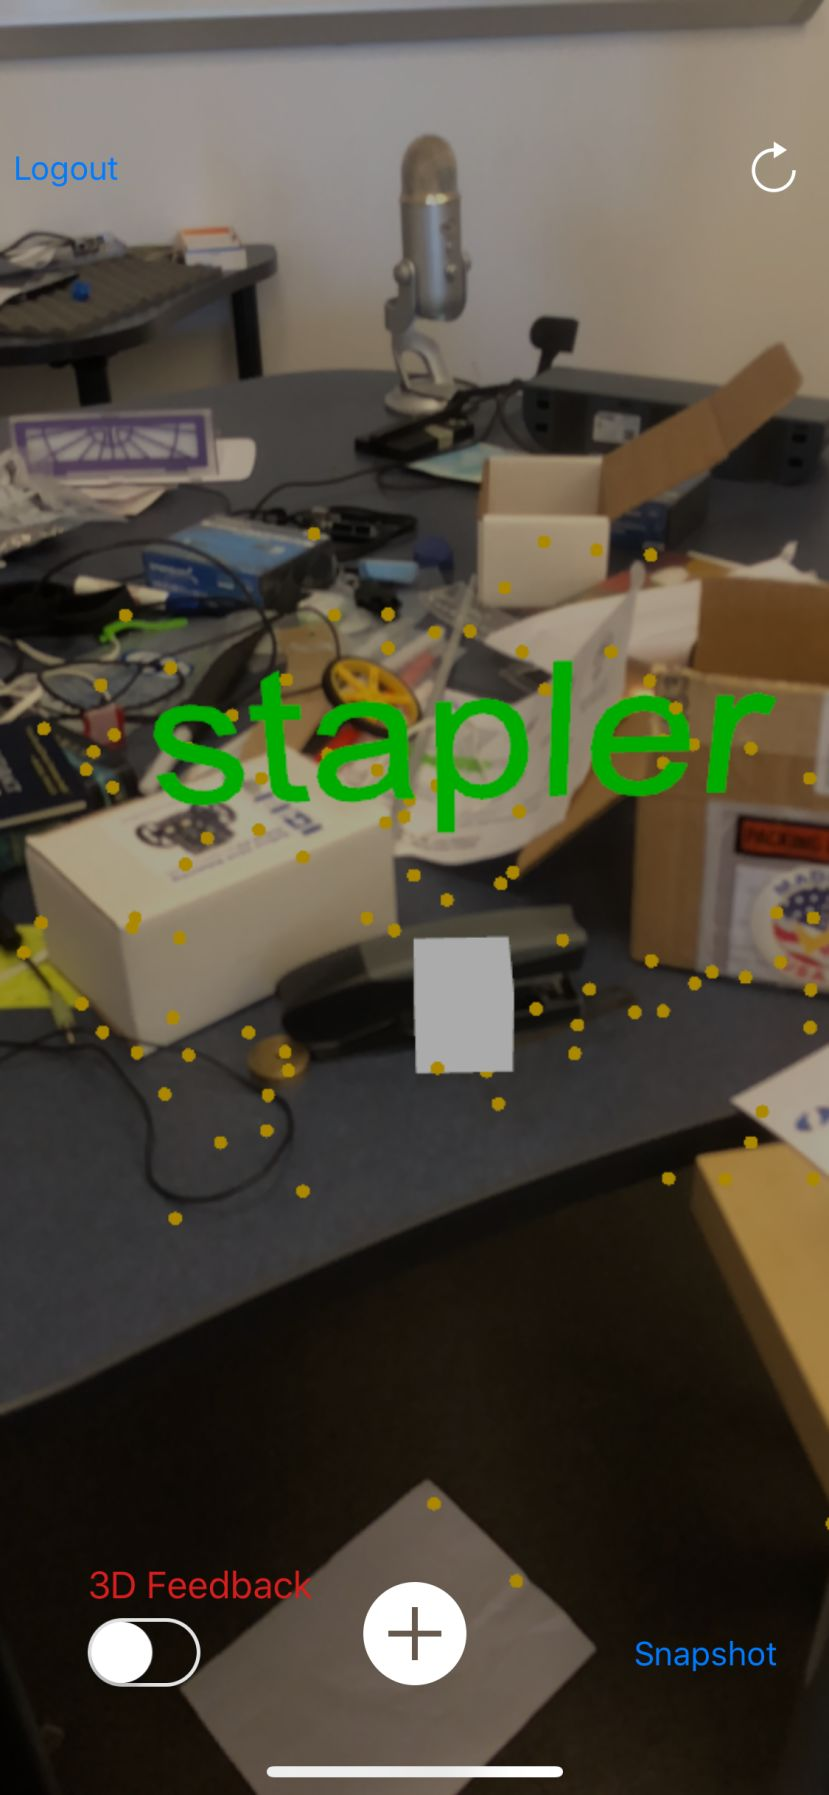
\includegraphics[height=3in]{Figures/viewshare_user}
\end{center}
\caption{Left image: the ViewShare interface for the crowdworker.  The crowdworker is instructed to locate the stapler in the series of images collected from the \BVI user's phone.  \textbf{Right image:} the interface for the \BVI user.  This interface shows a visualization of the location of the stapler as selected by the crowdworker.  While the visualization is not useful for user's who are blind, it is potentially useful for people who with low vision.  All elements of the interface are accessible via Apple's VoiceOver technology.\label{fig:viewsharescreenshots}}
\end{figure}


\subsection{2D to 3D Mapping}
In order to map a 2D pixel coordinate to a 3D point in space we utilize ARKit's built-in functionality for plane fitting.  We test the ray corresponding to the 2D pixel coordinate to see if it intersects a 3D plane (as determined by ARKit).  TODO a figure would be good here.  ARKit version 1.5, which we utilize for this study, is capable of finding both vertical and horizontal planes.  If the ray intersects a plane, we mark the object as localized and compute its 3D position using straightforward geometric formulas.  If the ray \emph{does not} intersect a known plane (either because the object located on a plane or because the plane has not been found by ARKit) we return an error condition to the volunteer.  In this situation, the volunteer must click on the object again from a second viewpoint.  Once the 2D pixel coordinate of the object is provided in two views, the ViewShare app uses triangulation to compute the 3D position.  The optimal 3D triangulation of two rays with endpoints $x_1$ and $x_2$ and unit directions $u_1$ and $u_2$ is given by the following equation.

\begin{align}
%c&= x_2 - x_1 \nonumber \\
%D &= x_1 + u_1 \frac{\left ( u_2 u_2^\top u_1  +  u_1   \right )^\top \left ( x_2 - x_1 \right) } {1 - \left ( u_1^\top u_2 \right)^2} \nonumber \\
%E &= x_2 + u_2 \frac{ \left ( u_1 u_2^\top u_1 - u_2 \right )^\top  \left ( x_2 - x_1 \right)  }{1 -  \left ( u_1^\top u_2 \right)^2} \nonumber \\
&\mbox{triangulate}(x_1, u_1, x_2, u_2) \nonumber = \\
&\frac{x_1 + x_2}{2}  + \frac{ u_1 u_1^\top u_2 u_2^\top  +  u_1 u_1^\top  + u_2 u_1^\top  u_2 u_1^\top - u_2 u_2^\top }{2 \left (1 -  \left ( u_1^\top u_2 \right)^2\right) } \left(  x_2 - x_1\right) \nonumber
\end{align}


%
%        let A = ray1.origin
%        let B = ray2.origin
%        let a = ray1.direction
%        let b = ray2.direction
%        let c = B - A
%        let D = A + a*(-simd_dot(a,b)*simd_dot(b,c)+simd_dot(a,c)*simd_dot(b,b))/(simd_dot(a,a)*simd_dot(b,b) - simd_dot(a,b)*simd_dot(a,b))
%        let E = B + b*(simd_dot(a,b)*simd_dot(a,c)-simd_dot(b,c)*simd_dot(a,a))/(simd_dot(a,a)*simd_dot(b,b) - simd_dot(a,b)*simd_dot(a,b))
%        let closestPoint = (D + E)/2

\subsection{Usability Study}
TBD

\subsection{Other Use Cases}
While we designed this app primarily for finding objects, it can also potentially be utilized for other tasks.  One major area of opportunity is finding things that are not objects (e.g., the precise location of a bus stop or doorway in outdoor settings where GPS is not sufficiently accurate.  A second major area of opportunity is automatically providing the location of relevant features in the environment (e.g., the locations of doors, windows, chairs) so that the user can make a mental map of the space around them.

\section{Discussion and Future Work}

\subsection{Future Work for the Clew and ViewShare Projects}
As stated earlier the basic version of the Clew app is already in the app store.  Beyond engaging with users deeply to understand how they experience the current version of the app and improving the usability based on their feedback, there are two major areas of future work we intend to explore.  The first is to improve the ability for the app to detect and communicate tracking failures.  When ARKit throws an error message, it is straightforward to communicate this information to the user, however, if the tracking drifts or becomes inaccurate without entering an error condition the user will be in a much more difficult situation.  In future versions of Clew we would like to be able to detect degraded tracking and alert the user.  A second area of future work would be to enable sharing of previously traveled routes with other Clew users.  This feature could work very similarly to the pause functionality where the user puts their phone in a known starting pose (e.g., against a door as they enter a building) which allows the phone to register its current location with the previously saved route.

For the ViewShare app there are many opportunities for future work.  A big theme to explore is the issue of quality control in crowdsourcing.  Aggregating judgments from multiple crowdworkers is a very active area of research in the machine learning community\todo{need citation} and applying some of these techniques to figure out whom to trust and how to filter out inaccurate localizations from the crowd would be immensely helpful.  A second area for future work is to test different use cases of this app (as mentioned earlier), including finding bus stops, doorways, or businesses in outdoor environments.

\subsection{Opportunities and Challenges in AR Assistive Apps}
The development of \emph{Clew} and \emph{ViewShare} provide useful information as to the potential of AR-based assistive apps.  The results demonstrate that for object finding --- within a room or on a tabletop --- and navigation along relatively short routes --- $~Xm$ --- the 3D motion estimation abilities of Apple's ARKit are sufficient for good performance.  As the complexity of the environment increase (either because it is larger or has few easily trackable features, which are essential for VIO to function well) other sources of information must be brought to bear on the problem.  For instance, in such cases external landmarks (e.g., signs, such as AprilTags, that are easily detectable in a phone's camera feed or Bluetooth Beacons) could be used to reduce tracking drift and provide anchors in the space.  A second method for adding robustness to AR-based apps would be to employ crowdsourcing to correct drift in the phone's motion estimates.  For example, a crowdworker might select the location of a particular  landmarks in images collected at two points in time so that drift in the system could be reduced.

\begin{enumerate}
\item Accessibility to voice over (minor problem, but worth mentioning.  Robust usability testing
\end{enumerate}
\balance{}

\section{Conclusion}
We have presented two smartphone apps that each allow people who are B/VI to perform significant, new tasks with their smartphones.  In contrast to the typical use cases of indoor navigation and image process where smartphones have provided significant value for users who are B/VI, our apps provide some of the first apps that can be used for navigation and object finding in arbitrary indoor environments.  While the initial results of our usability test are promising, much more work is required to refine the developed apps to be maximally useful to the B/VI community.

Further, we have outlined several promising areas of opportunity for the development of new augmented reality-enabled apps to support people who are B/VI.  We have also provided a discussion of the limitations of this technology.  With a combination of the development of new algorithms, careful co-design with users who are B/VI, and the improvement of the underlying AR capabilities from smartphone vendors these limitations can hopefully be overcome to create impactful new assistive smartphone technology for people who are B/VI.  

\section{Acknowledgments}
Removed for anonymous review.

% BALANCE COLUMNS

\newpage
% REFERENCES FORMAT
% References must be the same font size as other body text.
\bibliographystyle{SIGCHI-Reference-Format}
\bibliography{../references/assets,../references/assistive_tech,../references/disability_studies,../references/machine_learning}

\end{document}

%%% Local Variables:
%%% mode: latex
%%% TeX-master: t
%%% End:
